\chapter{State Estimation}
To give a better position estimate which can be fed to the controller as well, the different data collected from the sensors mounted are put through a \ac{KF}. This filter takes the different measurements as inputs to combine theese depending variance and different sample rate to give a better estimate of the position, rather than the quite noisy measurements taken using just the raw \ac{GPS} data directly.

To develop such a filter, the model of the ship is to be computed, as well as a mapping of the different inputs and outputs to the system. The model of the forward and sidewards case (surge and sway) are the same as for the discrete system. 

\subsection{State model}
The state model is used as a base for computing the influence the different inputs have on the system. The below formula is a general description for the state model of the system. 
\begin{align}
\vec{x}(k) = \vec{\Phi}(k)\vec{x}(k-1) + \vec{w}(k)
\end{align}
\noindent Where:
\begin{ffk}
$\vec{\Phi}(k)$ is the state matrix\\
$\vec{x}(k-1)$ is the last input to the system\\
$\vec{w}(k)$ is the driving noise (the system input)
\end{ffk}
In this case, the driving noise $\vec{w}(k)$ will be the inputs to the system, which can then be used to estimate the different states. The states to be estimated is the velocity $\dot{x}$, the angular velocity $\omega$ and the angle of the vessel in the local frame $\theta$. The driving noise (or input) can be defined as the $\vec{B}$ matrix in the state system, multiplied with the different inputs given to the system, namely $F(k)$ and $\tau(k)$, this changes the input (driving noise of the \ac{KF}) to $\vec{w}(k) = \vec{B} \vec{u}$ where $\vec{u}$ is a 2-by-1 vector with elements $F(k)$ and $\tau(k)$:
\begin{align}
\vec{x}(k) = \vec{\Phi}(k)\vec{x}(k-1) + \vec{w}(k)
\end{align}
The state model $\vec{\Phi}(k)$ can be seen as the same matrix 3-by-3 matrix inserted on the diagonal of a 9-by-9 matrix. This matrix expresses how an acceleration is turned into a position by defining the current position (or next) as a sum of the last position, the change due to the last velocity and the change due to the last acceleration, thus giving:
\begin{align}
\text{Pos}_x(k) = \text{Pos}_x(k-1) + \text{Vel}_x(k-1)\cdot ts +  \text{Acc}_x(k-1) \cdot \frac{ts^2}{2}
\end{align}
Using the same notation, it is possible to define the current velocity as:
\begin{align}
\text{Vel}_x(k) = \text{Vel}_x(k-1) + \text{Acc}_x(k-1) \cdot ts 
\end{align}
And finally define the acceleration as:
\begin{align}
\text{Acc}_x(k) = \text{Vel}_x(k-1)\cdot \beta_x(k-1) + \text{Acc}_x(k-1)
\label{eq:accx}
\end{align}
As the input to the system is an acceleration, the $\text{Acc}_x(k-1)$ term in equation \vref{eq:accx} is zeroed out, and is then input to the system via the input. These 3 formulas can be simplified and put on matrix form to make further computations easier, thus stating the state matrix as: 
\begin{align}
\vec{\Phi}_{X,Y,\omega}(k) = \begin{bmatrix}
1 & ts & \frac{ts^2}{2}\\
0 & 1 & ts\\
0 & -\beta _{X} & 0
\end{bmatrix}
\end{align}
Thus producing the state matrix as:
\begin{align}
\vec{\Phi}(k) = diag\{\vec{\Phi}_{X}(k),\vec{\Phi}_{Y}(k),\vec{\Phi}_{\omega}(k)\} 
\end{align}
$\vec{x}(k)$ is the state vector, and are given as:
\begin{align}
\vec{x}(k) = [x(k),\dot{x}(k),\ddot{x}(k),y(k),\dot{y}(k),\ddot{y}(k),\theta(k),\omega(k),\alpha(k)]^T
\end{align}
It is not all the available states we want to output, but the more inputs the system have, the better the estimate becomes. As stated, the input to the system is given as an acceleration. This can be defined as an input given as a force and an input given as a torque. The input can be defined as $\vec{u}(k)$ (the controller output) this is multiplied with an augmented version of the $\vec{B}$ matrix from the state space model $\vec{B}_a$ to transform it to an acceleration thus can $\vec{w}(k)$ be described by:
\begin{align}
\vec{w}(k) = \vec{B}_a\vec{u}(k) = \begin{bmatrix}
0 & 0 & \frac{1}{m} & 0 & 0 & 0 & 0 & 0 & 0\\
0 & 0 & 0 & 0 & 0 & 0 & 0 & 0 & \frac{1}{I}
\end{bmatrix}^T\begin{bmatrix}
F(k)\\
\tau(k)
\end{bmatrix}
\end{align}

\subsection{Observation model}
The observation model, is a model that models the different observations. In this case, the different observations are measured directly, as we can measure both the angular velocity, the angle and the velocity of the craft. The general formula for the observation model is given as:
\begin{align}
\vec{z}(k) = \vec{H}(k)\vec{x}(k) + \vec{v}(k)
\end{align}
\noindent Where:
\begin{ffk}
$\vec{H}(n)$ is the model linking the measurements to the observations\\
$\vec{v}(n)$ is the measurement noise on the sensors
\end{ffk}
The noise from the measurements is estimated using previous measurements which can be used to estimate the variance and the mean of the measurements. The noise can in general be seen as zero-mean Gaussian white noise processes, which makes for the assumption:
\begin{align}
\vec{v}(k) \sim \mathcal{N}(0,\sigma_v^2)
\end{align}
As $\vec{x}(n)$ is a row vector, $\vec{w}(n)$ is also a row vector with the same dimension. This calls for different variances on the different noise additions, for each of the measurements. As the variance of the noise on the \ac{IMU} is a lot bigger than on the \ac{GPS}. As all the measurements are available directly, the $\vec{H}(n)$ matrix is equal to identity. Giving the final observation model:
\begin{align}
\vec{z}(n) = \vec{x}(n) + \vec{v}(n)
\end{align}

% Wouldn't it be a fair assumption that a GPS doesn't have zero-mean, but has a wandering mean that would wander over time? 

% Text about the vector Kalman filer
% Text about the covariance matrix of such a system
\subsection{The Covariance matrices}
As the \ac{KF} in this project is a vector filter, the noise is added through covariance matrices:
\begin{align}
Cov(\vec{X},\vec{X}) = \text{E}\langle[\vec{X} - \vec{\mu}_X][\vec{X} - \vec{\mu}_X]^\text{T}\rangle \label{eq:covar}
\end{align}
The covariance matrix is used to tune the \ac{KF}, and weighs the different inputs according to the noise they experience. An assumption is to keep this constant. For the vector \ac{KF} there are two noises added to the system, one depicts the measurement noise, and the other the system noise. The system noise is in this project considered the input to the system. This can therefore be seen as the covariance of the input signals to the ship. As seen in \todo{insert reference to worksheet once its done -rlc} the distributions of the input signal $\vec{u}(k)$ can be seen as:
\begin{align}
F \sim \mathcal{N}(5.3544,55)\\
\tau \sim \mathcal{N}(0,20)
\end{align}
As the two inputs are independent, the covariance matrix collapses to a matrix with diagonal entries, which gives the following matrix for the system covariance. 
\begin{align}
Cov(\vec{w}(k),\vec{w}(k))_{3,3} &= \sigma_{Fx}^2\\
Cov(\vec{w}(k),\vec{w}(k))_{6,6} &= \sigma_{Fy}^2\\
Cov(\vec{w}(k),\vec{w}(k))_{9,9} &= \sigma_{\tau}^2
\end{align}
The measurement covariance is also given as a diagonal matrix as all the entries herein is given as the variance of the individual signals. These variances are estimated in \todo{insert reference to Juuls document -rlc} and the covariance matrix then becomes:
\begin{align}
Cov(\vec{v}(k),\vec{v}(k)) = diag\{\sigma_{x}^2,\sigma_{\dot{x}}^2,\sigma_{\ddot{x}}^2,\sigma_{y}^2,\sigma_{\dot{y}}^2 = 0,\sigma_{\ddot{y}}^2,\sigma_{\theta}^2,\sigma_{\omega}^2,\sigma_{\alpha}^2 = 0\}
\end{align}

\section{\ac{KF} description}
The \ac{KF} can be divided into two steps, an update step and a prediction step. The update step updates all the variables, while the prediction step does the actual prediction. This is carried out using 
\begin{align}
\vec{x}(k) &= \vec{\Phi}(k)\vec{x}(k-1) + \vec{w}(k)\\
\vec{z}(k) &= \vec{H}(k)\vec{x}(k) + \vec{v}(k)\\
\hat{\vec{x}}(k)_{(-)} &= \vec{\Phi}(k-1)\hat{\vec{x}}(k-1)_{(+)}\\
\vec{P}(k)_{(-)} &= \vec{\Phi}(k-1) \vec{P}(k-1)_+ \vec{\Phi}(k-1)^T + \vec{Q}(k-1)\\
\hat{\vec{x}}(k)_{(+)} &= \hat{\vec{x}}(k)_{(-)} + \bar{\vec{K}(k)}[\vec{z}(k) - \vec{H}(k)\cdot\hat{\vec{x}}(k)_{(-)}]\\
\vec{P}(k)_{(+)}&= [\vec{I} - \bar{\vec{K}(k)}\vec{H}(k)]\vec{P}(k)_{(-)}\\
\bar{\vec{K}(k)} &= \vec{P}(k)_{(-)} \vec{H}(k)^T [\vec{H}(k)\vec{P}(k)_{(-)} \vec{H}(k)^T + \vec{R}(k)]^{-1}
\end{align}
\noindent Where
\begin{ffk}
$\hat{\vec{x}}(k)_{(-)}$ = Predicted step of $\vec{x}(k)$\\
$\vec{P}(k)_{(-)}$ = Prediction of the covariance\\
$\hat{\vec{x}}(k)_{(+)}$= Estimate of the state\\
$\vec{P}(k)_{(+)}$ = Update of the covariance\\
$\bar{\vec{K}(k)}$ = Kalman gain with $\vec{\Lambda}$ multiplied onto it
\end{ffk}

\section{Simulations of the \ac{KF}}
Through simulations, the covariance matrices have been determined, as a dynamic covariance matrix have produced some bad results. When the system is simulated with a $sin(\theta)$ (0.2 amplitude, 0.001 Hz) angle reference and a $1$ m/s velocity reference using the \MATLAB  script found on the CD-rom for 5000 samples , the system produces the below figure \vref{fig:kalmanA}. All the figures below are zoomed in on the tip of the track, where the biggest error is expected as this is where the ship turns. 


When the system is simulated it gives the following response for estimating the position.
\begin{figure}[htbp]
	\centering
	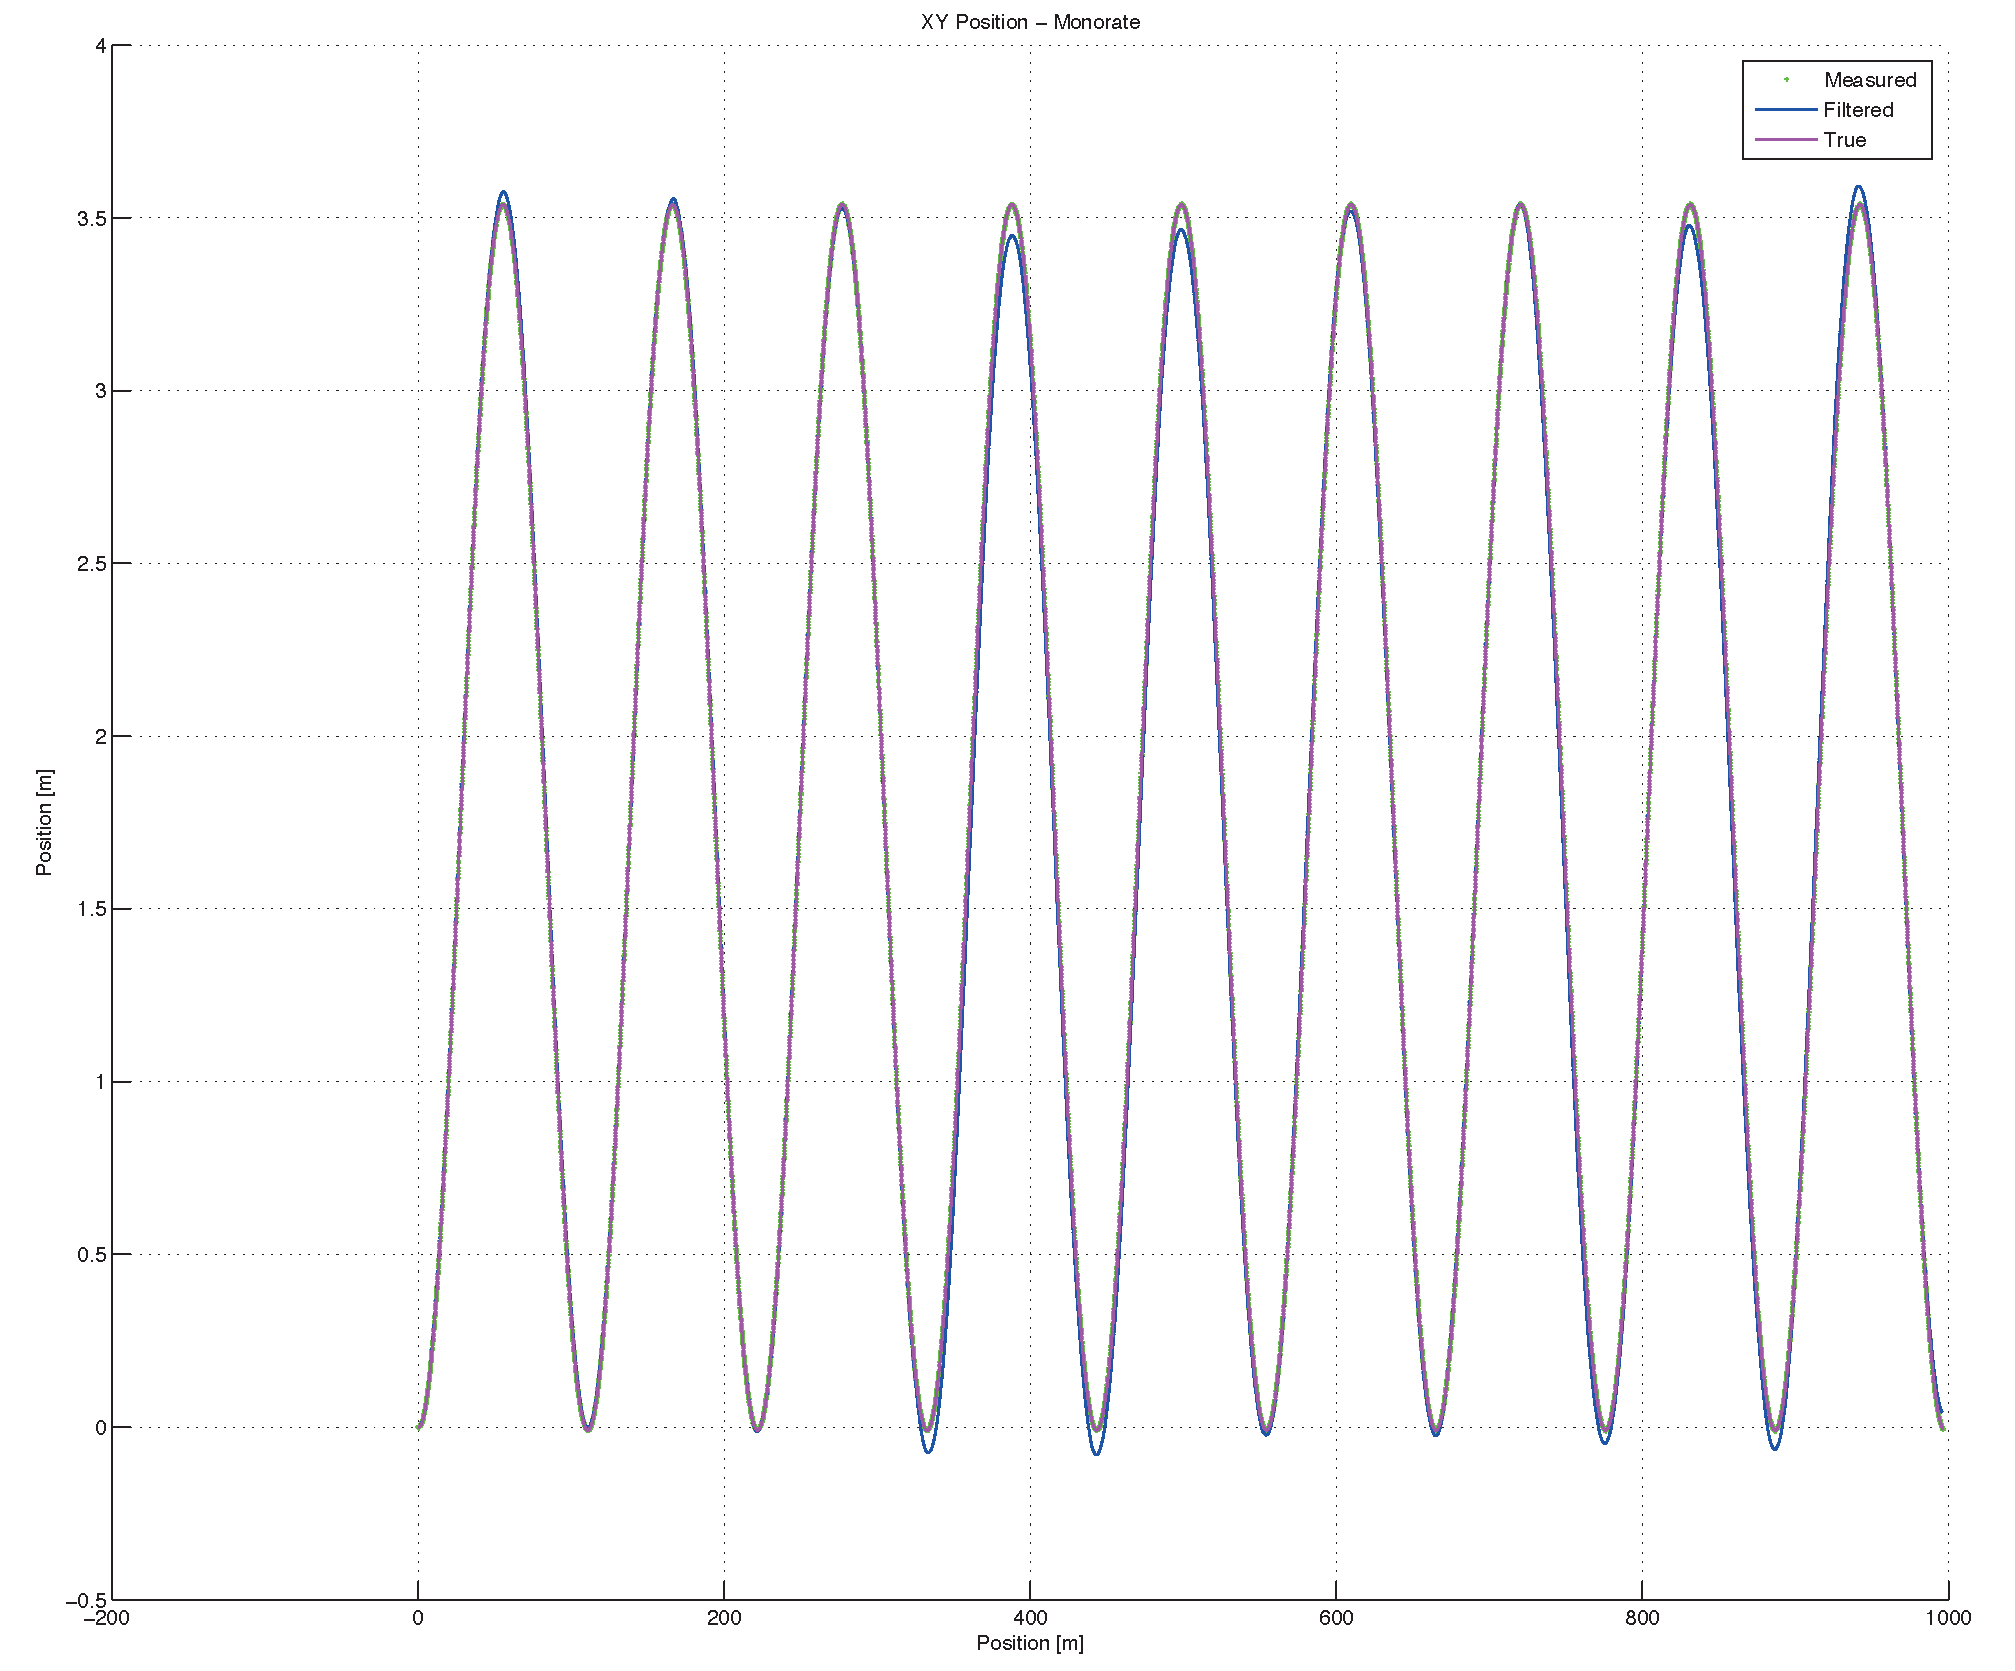
\includegraphics[width=\textwidth]{img/kalmana}
	\caption{Simulation of the \ac{KF} with reference signal given as: 1 m/s and angle as $sin(\theta)$, with 0.2 amplitude and 0.001 Hz frequency for 5000 samples. The two sensors samples at 10 Hz.}
	\label{fig:kalmanA}
\end{figure}

Figure\vref{fig:kalmanA} depicts the output of the \ac{KF} when the sampling rate of the \ac{GPS} and the \ac{IMU} are equal. However on the actual system - the \ac{GPS} only samples at 1 Hz and the \ac{IMU} samples at 10 Hz, the filter needs to be changed. The \ac{KF} must account for this change, which can be done by setting the noise of the measurement to a high value, which in turn will reduce the Kalman gain $\bar{\vec{K}(k)}$ to zero. Another implementation would be to zero the gain manually. This produces the below figure \vref{fig:kalmanB} as a function of the \ac{GPS} being sampled only once every second, while the \ac{IMU} is sampled at 10 Hz. 

\begin{figure}[htbp]
	\centering
	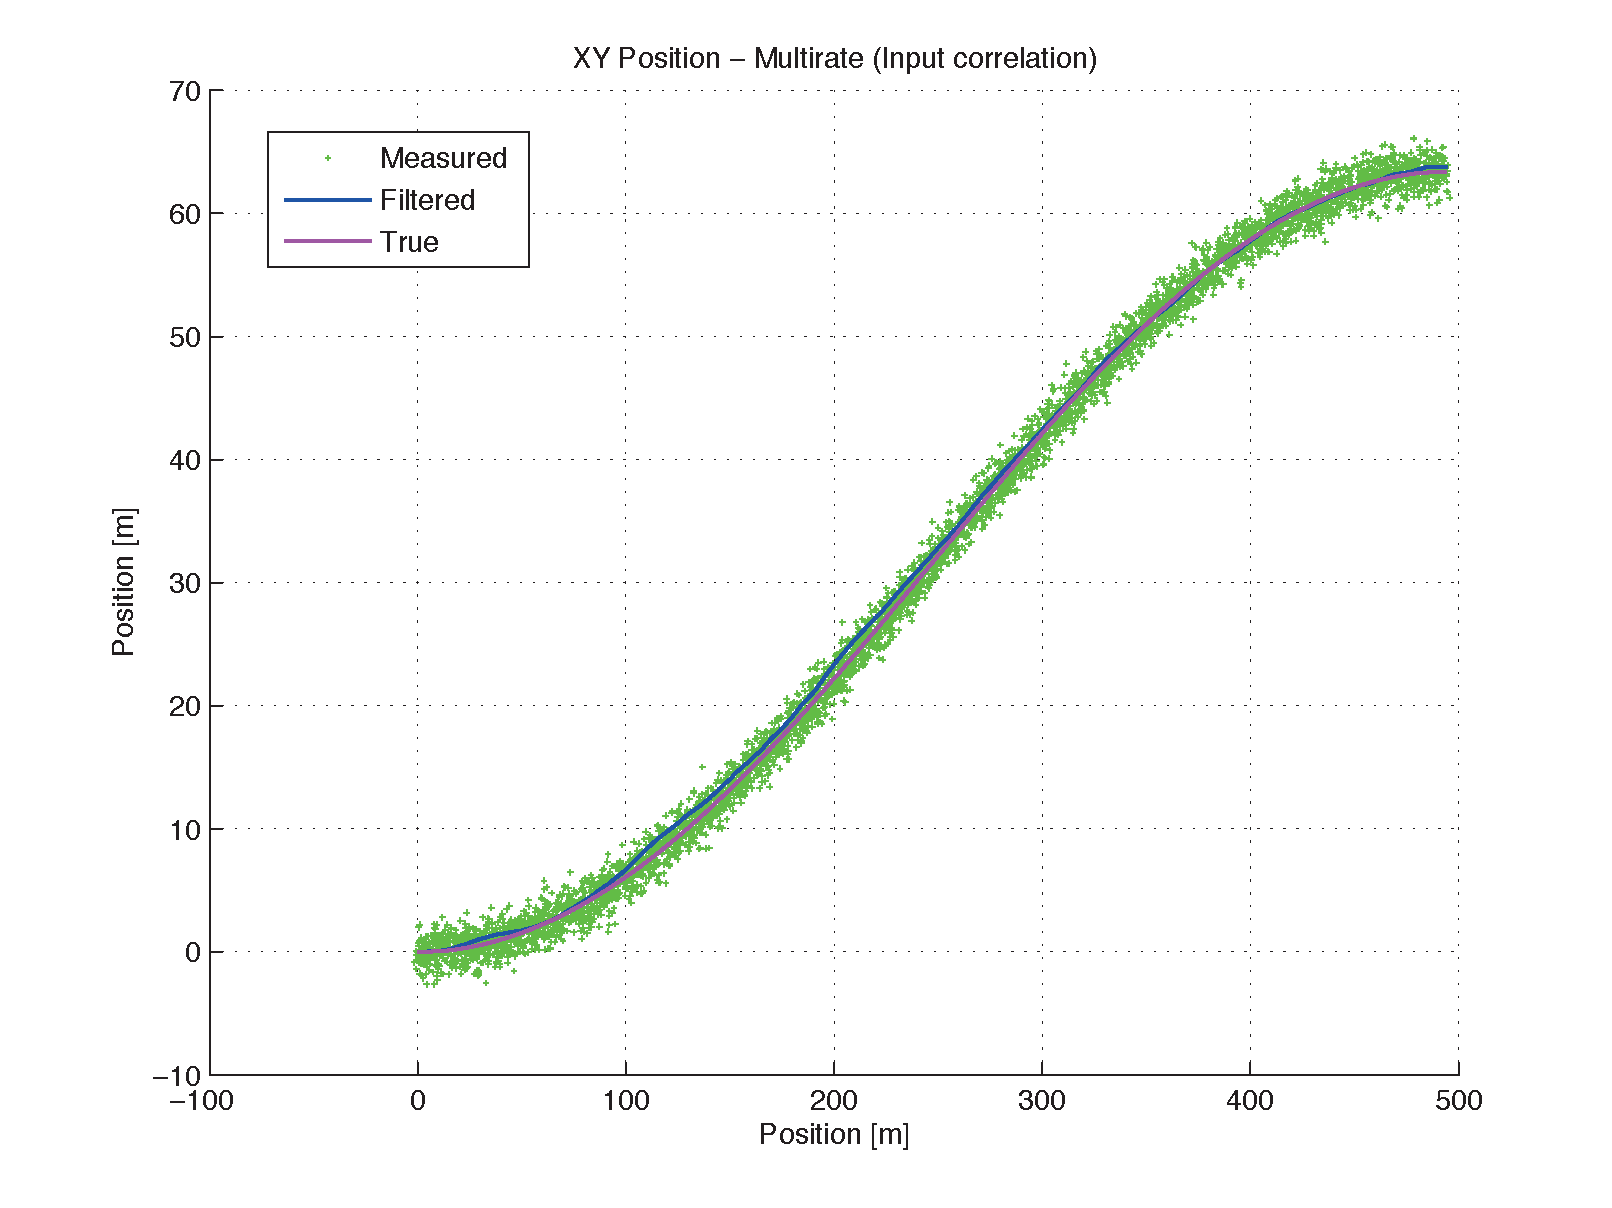
\includegraphics[width=\textwidth]{img/kalmanb}
	\caption{Simulation of the \ac{KF} with reference signal given as: 1 m/s and angle as $sin(\theta)$, with 0.2 amplitude and 0.001 Hz frequency for 10000 samples. The system gains the measurements when no \ac{GPS} amples are present with 0.}
	\label{fig:kalmanB}
\end{figure}

If the Kalman gain $\bar{\vec{K}(k)}$ is not zeroed out, the \ac{KF} will use the same sample as input, this causes the filter to try and make the system converge towards the last known value. If this is simulated it produces the following plot shown on \vref{fig:kalmanC}:

\begin{figure}[htbp]
	\centering
	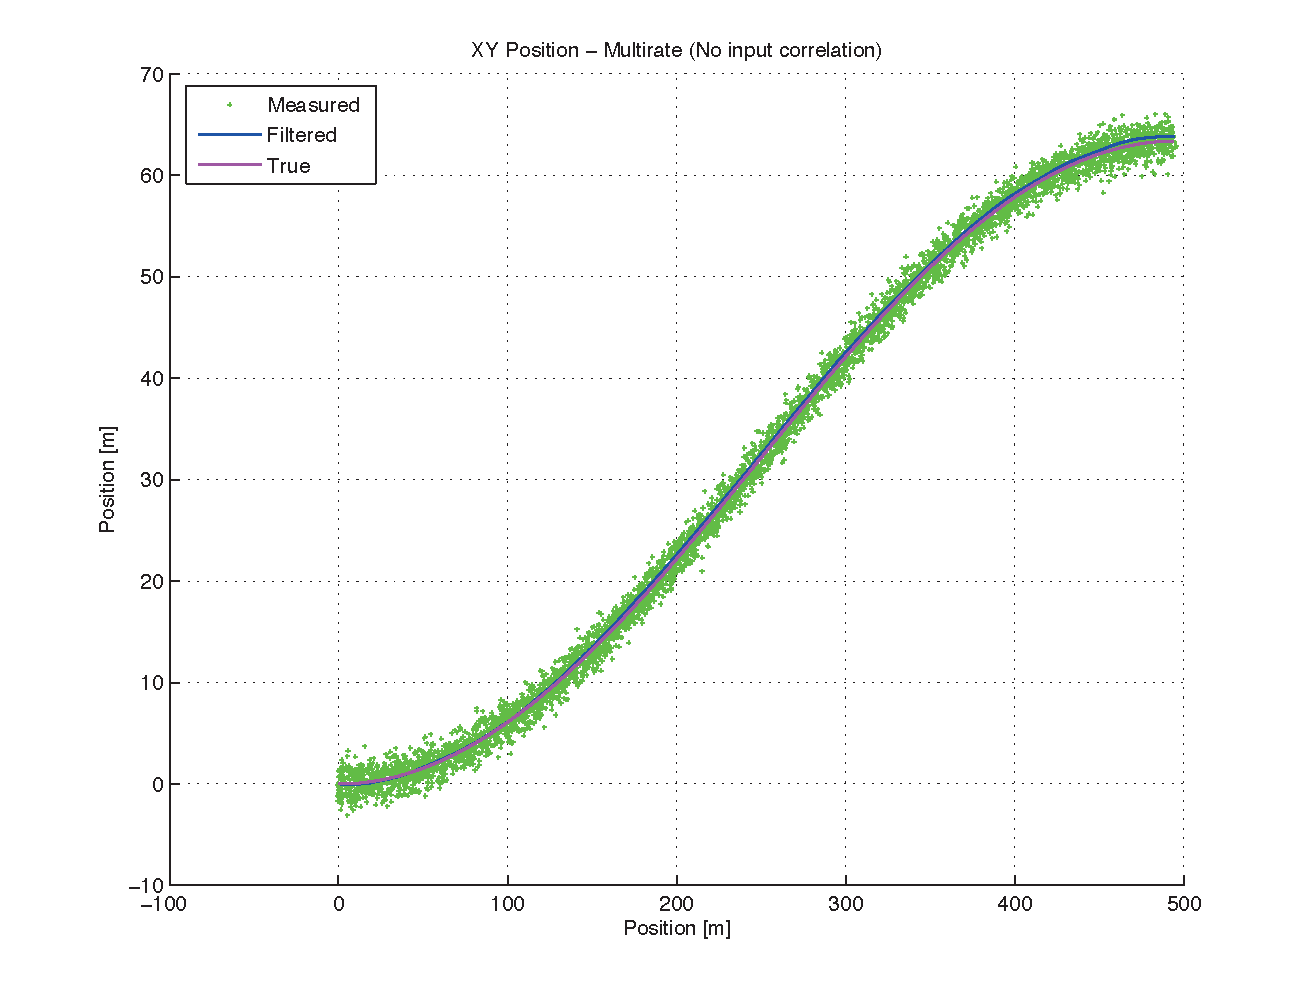
\includegraphics[width=\textwidth]{img/kalmanc}
	\caption{Simulation of the \ac{KF} with reference signal given as: 1 m/s and angle as $sin(\theta)$, with 0.2 amplitude and 0.001 Hz frequency for 5000 samples. The system sets the current \ac{GPS} measurement equal the last when no new sample is present.}
	\label{fig:kalmanC}
\end{figure}

\subsection{Simulations of the filter}
Below is 3 plots of the \ac{KF} running with a square pulse input as the angle reference. Figure \vref{fig:xymono} depicts the system running when the sensors are running at the same sampling frequency. On the box on the plot the estimate clearly converges and follows the actual path nicely. 

\begin{figure}[htbp]
	\centering
	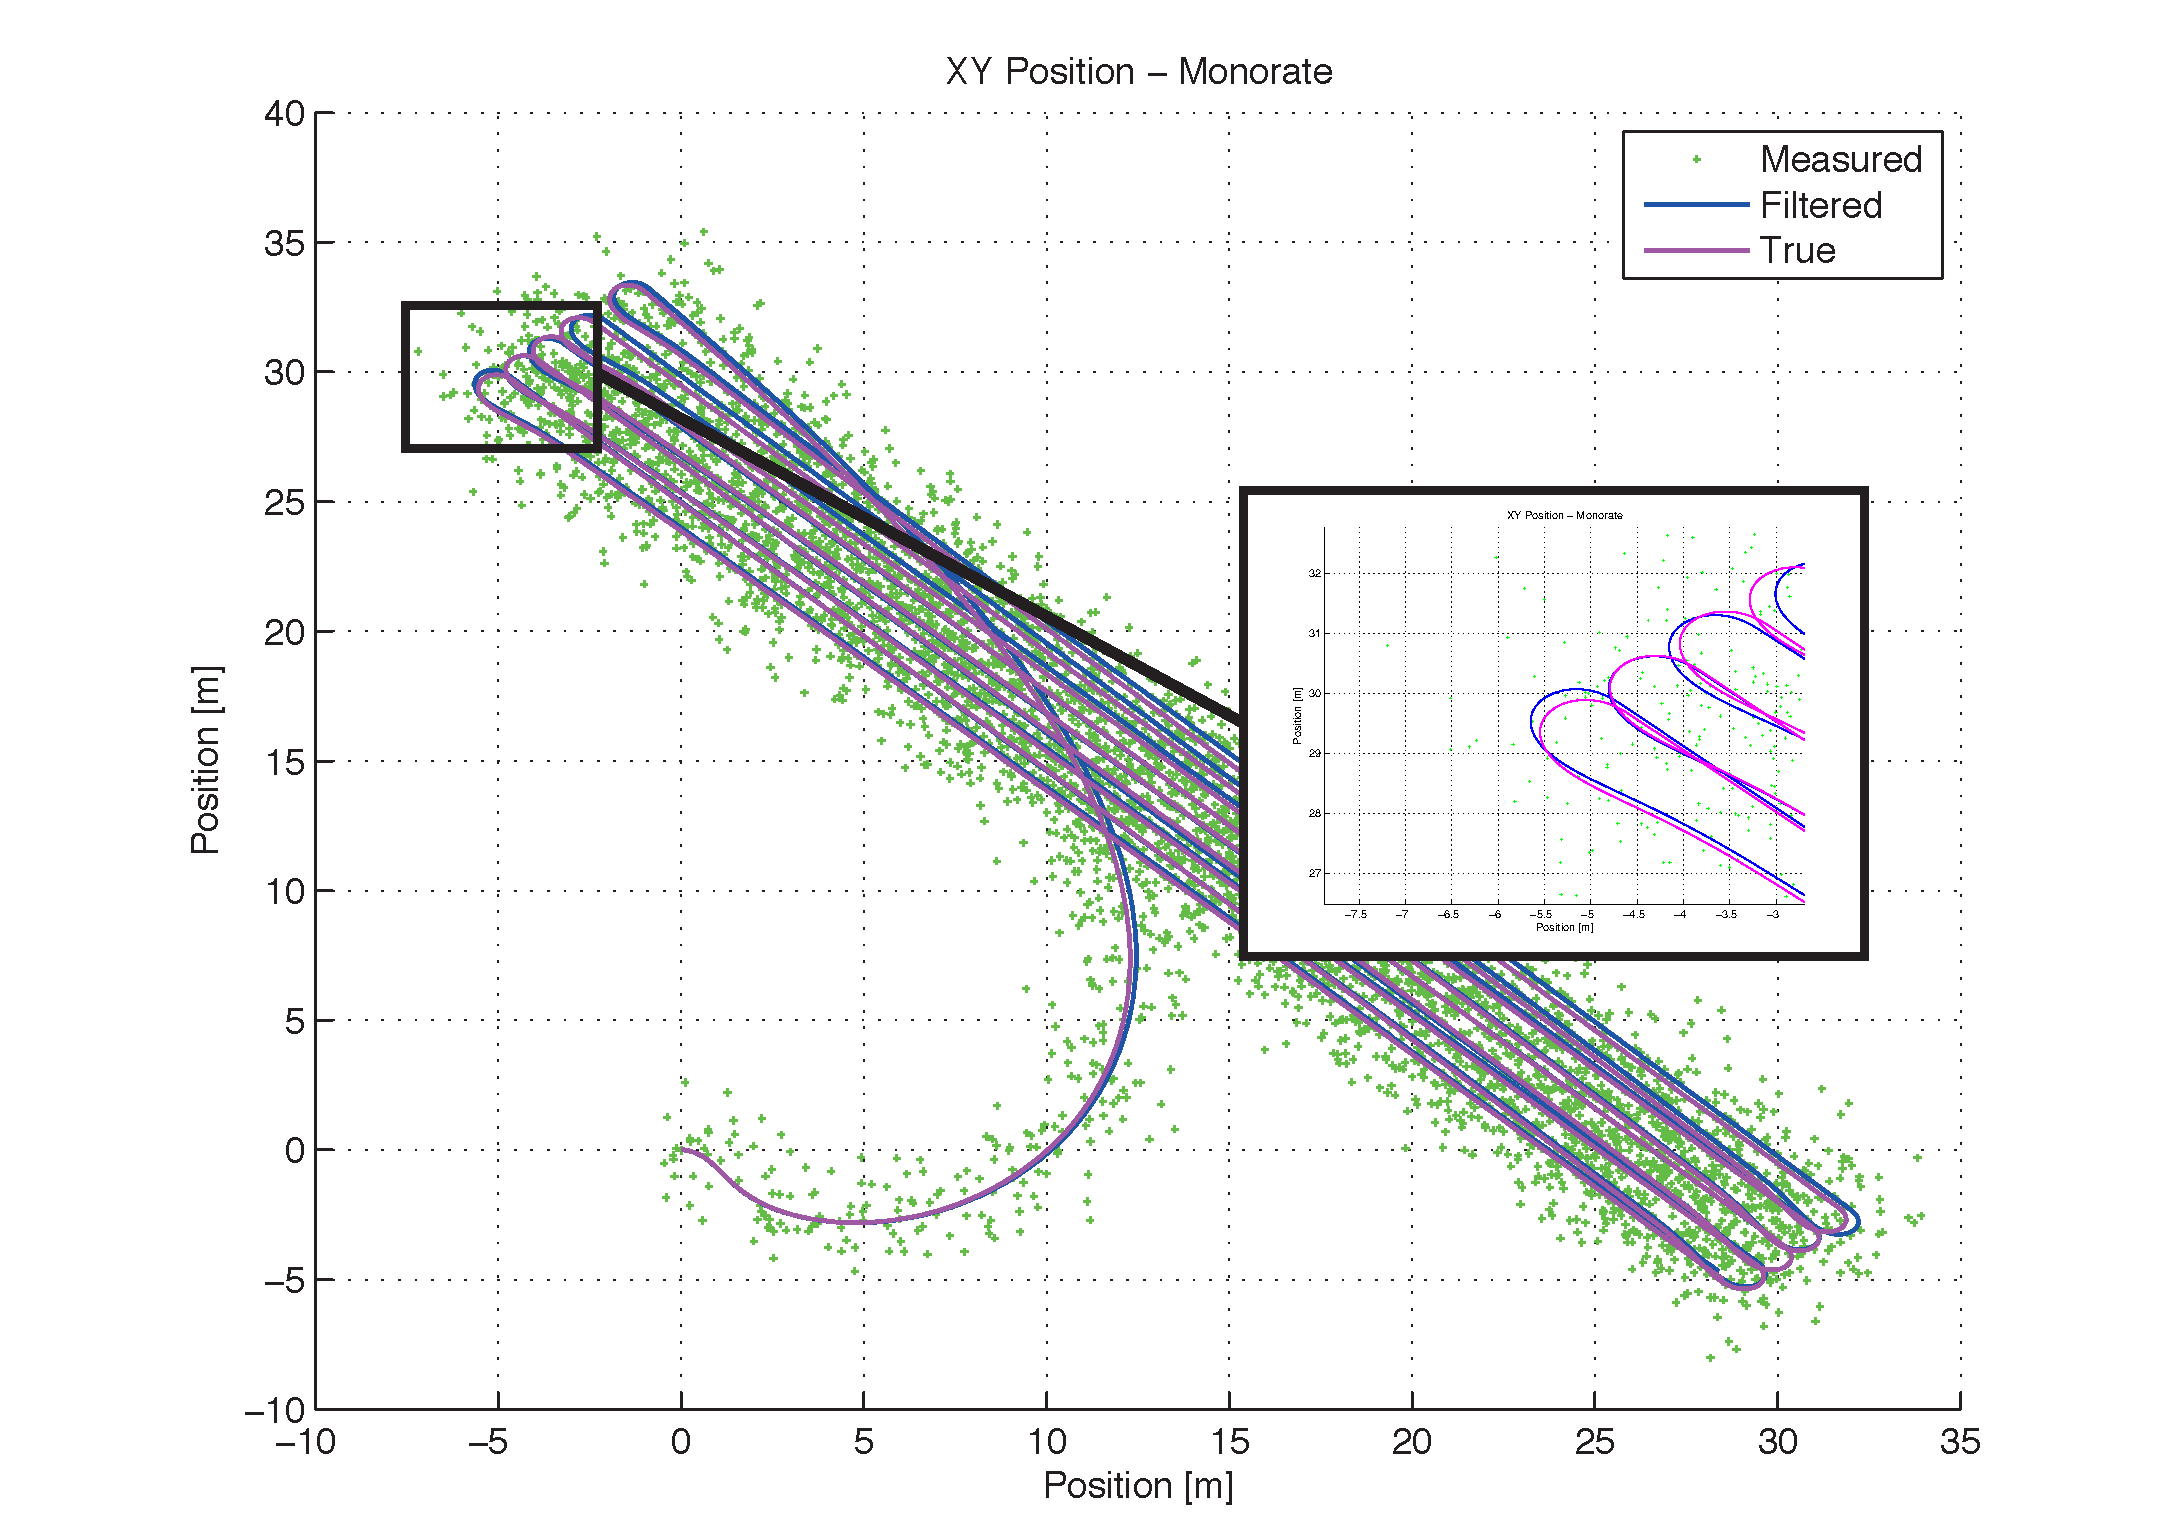
\includegraphics[width=\textwidth]{img/xymono}
	\caption{Simulation of the \ac{KF} with the same sampling rate on the sensors}
	\label{fig:xymono}
\end{figure}

On \vref{fig:xymulti1} the sampling rates are different and the Kalman gain $\bar{\vec{K}(k)}$ is set to zero when no new \ac{GPS} sample is present. This also tracks the true path very nicely, but varies a little more. 

\begin{figure}[htbp]
	\centering
	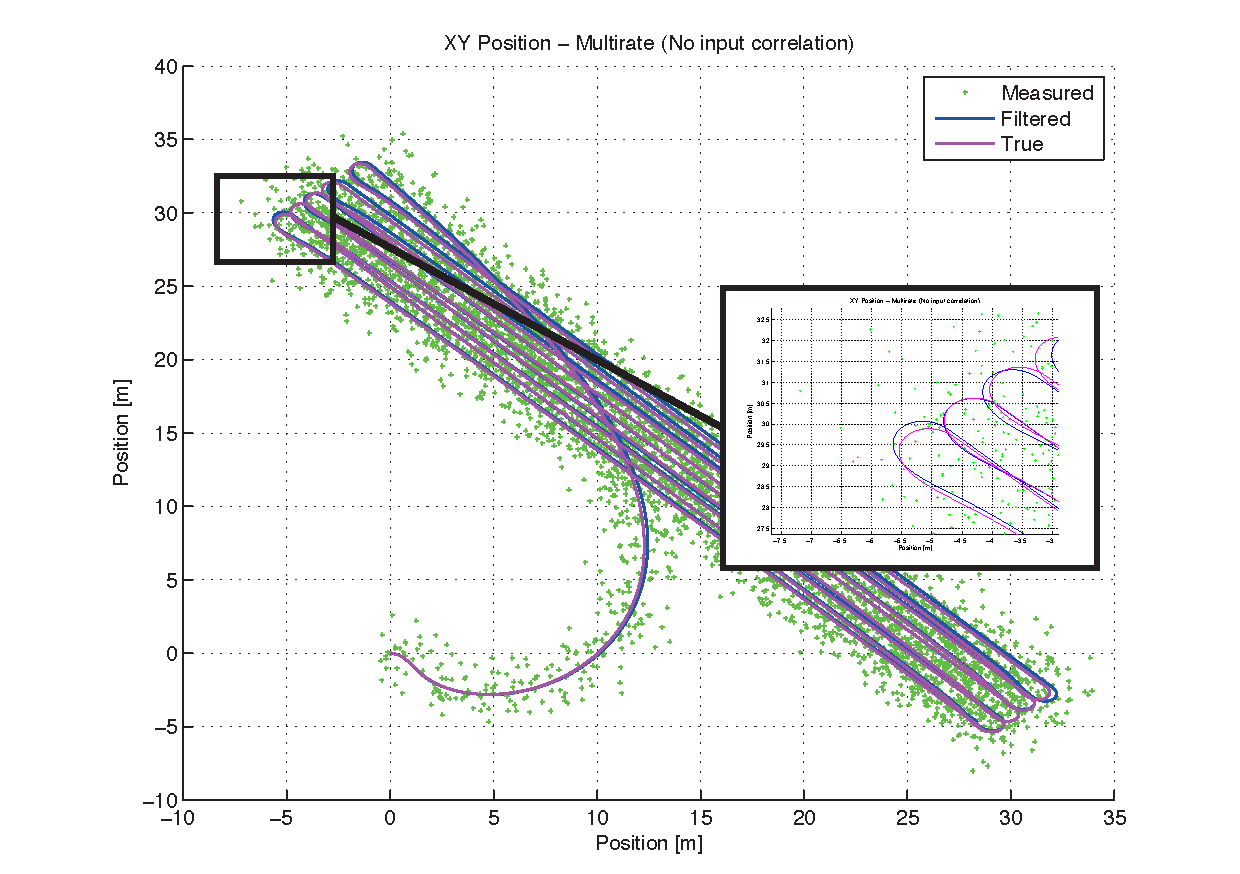
\includegraphics[width=\textwidth]{img/xymultirate}
	\caption{Simulation of the \ac{KF} with the \ac{IMU} running at 10 Hz and the \ac{GPS} at 1 Hz}
	\label{fig:xymulti1}
\end{figure}

The last figure \vref{fig:xymulti2} depicts the system where the input is only updated once every second. And this causes the system to diverge, but then pick up the lost sample again, thus making for a system that slowly will diverge.

\begin{figure}[htbp]
	\centering
	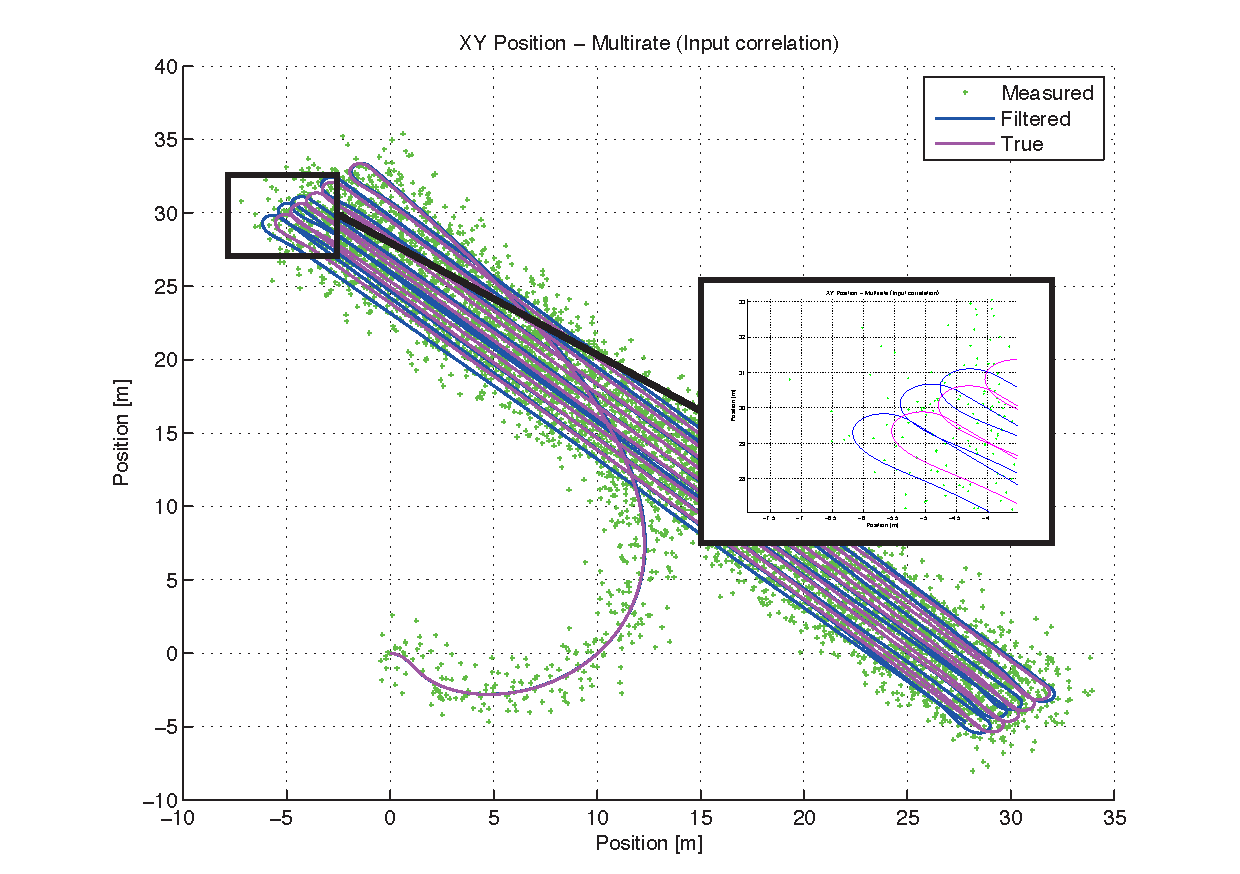
\includegraphics[width=\textwidth]{img/xymnirate}
	\caption{Simulation of the \ac{KF} with the \ac{IMU} running at 10 Hz and the \ac{GPS} at 1 Hz - but converging towards the old sample}
	\label{fig:xymulti2}
\end{figure}

\section{Position estimation}
During the development of the \ac{KF} a lot or problems were discovered. One is to estimate the variances of the different measurement devies. The GPS delivers a position in latitude longitude format - which is converted into an x and y coordinate by rotating the entire system and shifting the local frame of the ship as a surface tangent to the earth. This will of course only be an estimate, but as the curvature of the earth is relatively small. The distance to the horizon can be estimated by $d \approx 3.57\sqrt{h}$ which on the ground, equals that the distance to the horizon is approximately 3.57 kilometers. As the areas to be measured are defined by a local bounding box - this area will to be defined to be smaller than 3.5 kilometers.

This section will contain the different things we've considered during the miniproject in \ac{KF}ing, and will be used to give a better estimate of the actual position (from the measurements implemented on the ship).

Below is a description of the measurable inputs to the system. These are obtained from a \ac{GPS} and a \ac{IMU} mounted on the ship.
Position and velocity from the \ac{GPS}: rotated coordinates (from LatLon to Local frame)
Linear acceleration from the \ac{IMU}: accelerometer
Angular acceleration from the \ac{IMU}: gyrometer
Angle from the \ac{IMU}: magnetometer (compass)

\section{Estimation of position on a lossy channel}
As the controls are run on a remote platform, the \ac{KF} should be able to work even though some sensor measurements are corrupted. To work around this, the Kalman gain should be set to zero of the readout is corrupted - so every time the receiver gets a packet where the checksom is invalid, it generates a matrix mask that tells which rows of the Kalman gain should be zeroed, the mask is defined as:

\begin{align}
\vec{\Lambda} = diag\{\lambda_x,\lambda_{\dot{x}},\lambda_{\ddot{x}},\lambda_{\lambda{y}},\lambda_{\dot{y}},\lambda_{\ddot{y}},\lambda_{\theta},\lambda_{\omega},\lambda_{\alpha} \}
\end{align}
\noindent Where the individual $\lambda$'s is given as: 
\begin{align}
\lambda = 
\left\{ 
  \begin{array}{l l}
    1 & \quad \text{if measurement is valid}\\
    0 & \quad \text{otherwise}
  \end{array} \right.
\end{align} 
Thus augmenting the Kalman gain $\bar{\vec{K}(k)}$ equations to:
\begin{align}
\bar{\vec{K}(k)} &= \langle\vec{P}(k)_{(-)} \vec{H}(k)^T [\vec{H}(k)\vec{P}(k)_{(-)} \vec{H}(k)^T + \vec{R}(k)]^{-1}\rangle\vec{\Lambda} 
\end{align} 

To test this, \MATLAB has been used, which generates the the following results for a given packet loss rate. This rate can be then be altered to see how the system responds to a given data loss rate. The data loss rate is given in percent. If the system looses 10\% of the packages, the following error curves of the absolute position error is produced

The 6 figures represent the error with a 0.1 percent loss, a 1 percent loss, 5 percent loss, a 10 percent loss, a 15 percent loss and finally a 20 percent loss. 

\section{Implementation of the \ac{KF}}
The \ac{KF} is implemented in Python and is run on the \ac{HLI}. On the implementation it self, the \ac{KF} is fed the control signals measured. A depiction of the actual implementation is seen on figure \vref{fig:kalmanimp}.

\begin{figure}[htbp]
	\centering
	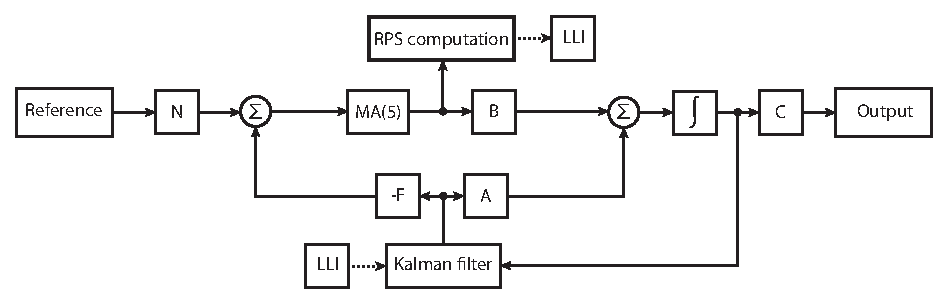
\includegraphics[width=\textwidth]{img/kalmanim}
	\caption{Depiction of the \ac{KF} implementation. The \ac{KF} is used to estimate the measurements more precisely.}
	\label{fig:kalmanimp}
\end{figure}
